\documentclass{standalone}

\usepackage{tikz}
\usepackage{pgfplots}
\usepgfplotslibrary{statistics}
\usetikzlibrary{pgfplots.statistics}
\usepackage{etoolbox}

\newtoggle{label}
\togglefalse{label}

\pgfplotsset{compat=1.12}

\begin{document}
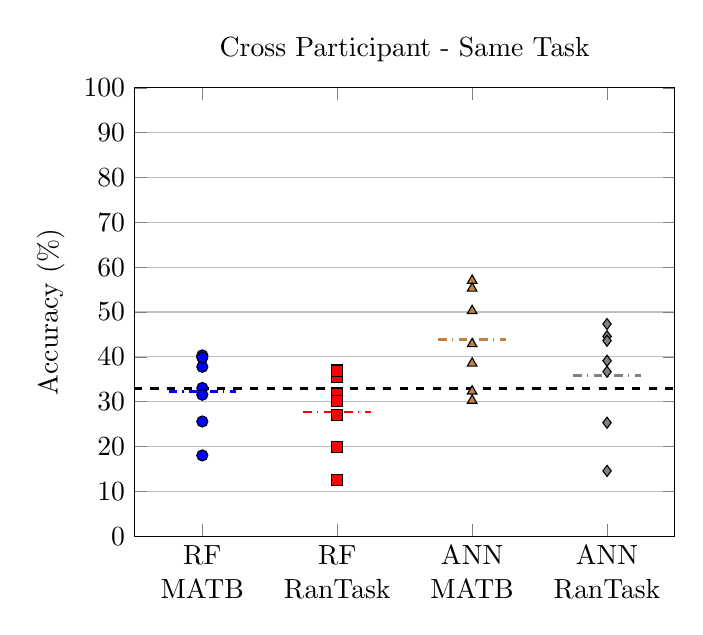
\begin{tikzpicture}
\begin{axis}[
	ymajorgrids,
	scatter/classes= {
		a={mark=*, fill=blue, draw=black},
		b={mark=square*, fill=red, draw=black},
		c={mark=triangle*, fill=brown, draw=black},
		d={mark=diamond*, fill=gray, draw=black}
	},
	ymin=0,
	ymax=100,
	xmin = .5, 
	xmax=4.5,
	ytick={0,10,...,100},
	xtick={1,2,3,4},
	xticklabel style={align=center},
	xticklabels={RF\\MATB, RF\\RanTask, ANN\\MATB, ANN\\RanTask},
	title=Cross Participant - Same Task, 
	ylabel=Accuracy (\%)]

\addplot+[ mark=None, dashed, black, line width = 1pt ]
	coordinates {
	(0, 33)
	(5, 33)	
};

	% Random Forest MATB
	\addplot+[ scatter,
			only marks,
			scatter src=explicit symbolic]
	coordinates {
			(1, 25.59) [a]
			(1, 37.78) [a]
			(1, 18.02) [a]
			(1, 33.05) [a]
			(1, 40.33) [a]
			(1, 39.83) [a]
			(1, 31.55) [a]
};

% Random Forest MATB Mean
	\addplot+[ mark=None, dashdotted, blue, line width = 1pt ] 
	coordinates {
		(0.75, 32.30)
		(1.25, 32.30)
};


	% Random Forest RanTask
	\addplot+[ scatter,
			only marks,
			scatter src=explicit symbolic]
	coordinates {
			(2, 35.57) [b]
			(2, 12.46) [b]
			(2, 19.97) [b]
			(2, 27.06) [b]
			(2, 36.94) [b]
			(2, 31.83) [b]
			(2, 30.23) [b]
};
% Random Forest MATB Mean
	\addplot+[ mark=None, dashdotted, red, line width = 1pt ] 
	coordinates {
		(1.75, 27.72)
		(2.25, 27.72)
};


	% ANN MATB
	\addplot+[ scatter,
			only marks,
			scatter src=explicit symbolic]
	coordinates {
			(3, 32.34) [c]
			(3, 57.02) [c]
			(3, 30.28) [c]
			(3, 42.89) [c]
			(3, 55.28) [c]
			(3, 50.28) [c]
			(3, 38.56) [c]
};
% Random Forest MATB Mean
	\addplot+[ mark=None, dashdotted, brown, line width = 1pt ] 
	coordinates {
		(2.75, 43.80)
		(3.25, 43.80)
};


	% ANN RanTask
	\addplot+[ scatter,
			only marks,
			scatter src=explicit symbolic]
	coordinates {
			(4, 36.69) [d]
			(4, 14.56) [d]
			(4, 25.31) [d]
			(4, 39.13) [d]
			(4, 44.57) [d]
			(4, 47.32) [d]
			(4, 43.60) [d]
};
% Random Forest MATB Mean
	\addplot+[ mark=None, dashdotted, gray, line width = 1pt ] 
	coordinates {
		(3.75, 35.88)
		(4.25, 35.88)
};



\end{axis}
\end{tikzpicture}

\end{document}
















